The previous chapter looked at persistent memory programming from the perspective of consistency models and programming interfaces.
While necessary to define correct program behavior, I did not consider actual implementations or investigate specific optimizations.
This chapter investigates performance more directly, considering two simple persistent programming patterns -- a persistent log/buffer and a persistent linked list.
While I will describe how I expect the persistent memory consistency models from the previous chapters operate with each pattern, the point is to highlight potential performance bottlenecks and necessary optimizations.
I do not yet consider actual programming models or hardware to provide many of these optimizations.

Prior work has examined building data structures for NVRAM.
However, these works generally address other issues such as write endurance \cite{ChenGibbons11}, suggest data structures that intuitively fit NVRAM's programming interface without concern for performance \cite{VenkataramanTolia11}, or propose complicated software mechanisms to work around incomplete or inferior persistent consistency models \cite{FangHsiao11}.
While BPFS \cite{ConditNightingale09} takes a more holistic approach, their model falls short in terms of correctness, multi-threaded performance, and possibly single-thread performance, as I will show shortly.
I take a different approach, looking at useful data structures and potential performance concerns and using this insight to imagine new persistent consistency models and optimizations.

\section{Persistent Buffer}
\label{sec:PMC_patterns:Buffer}

\begin{figure}
\centering
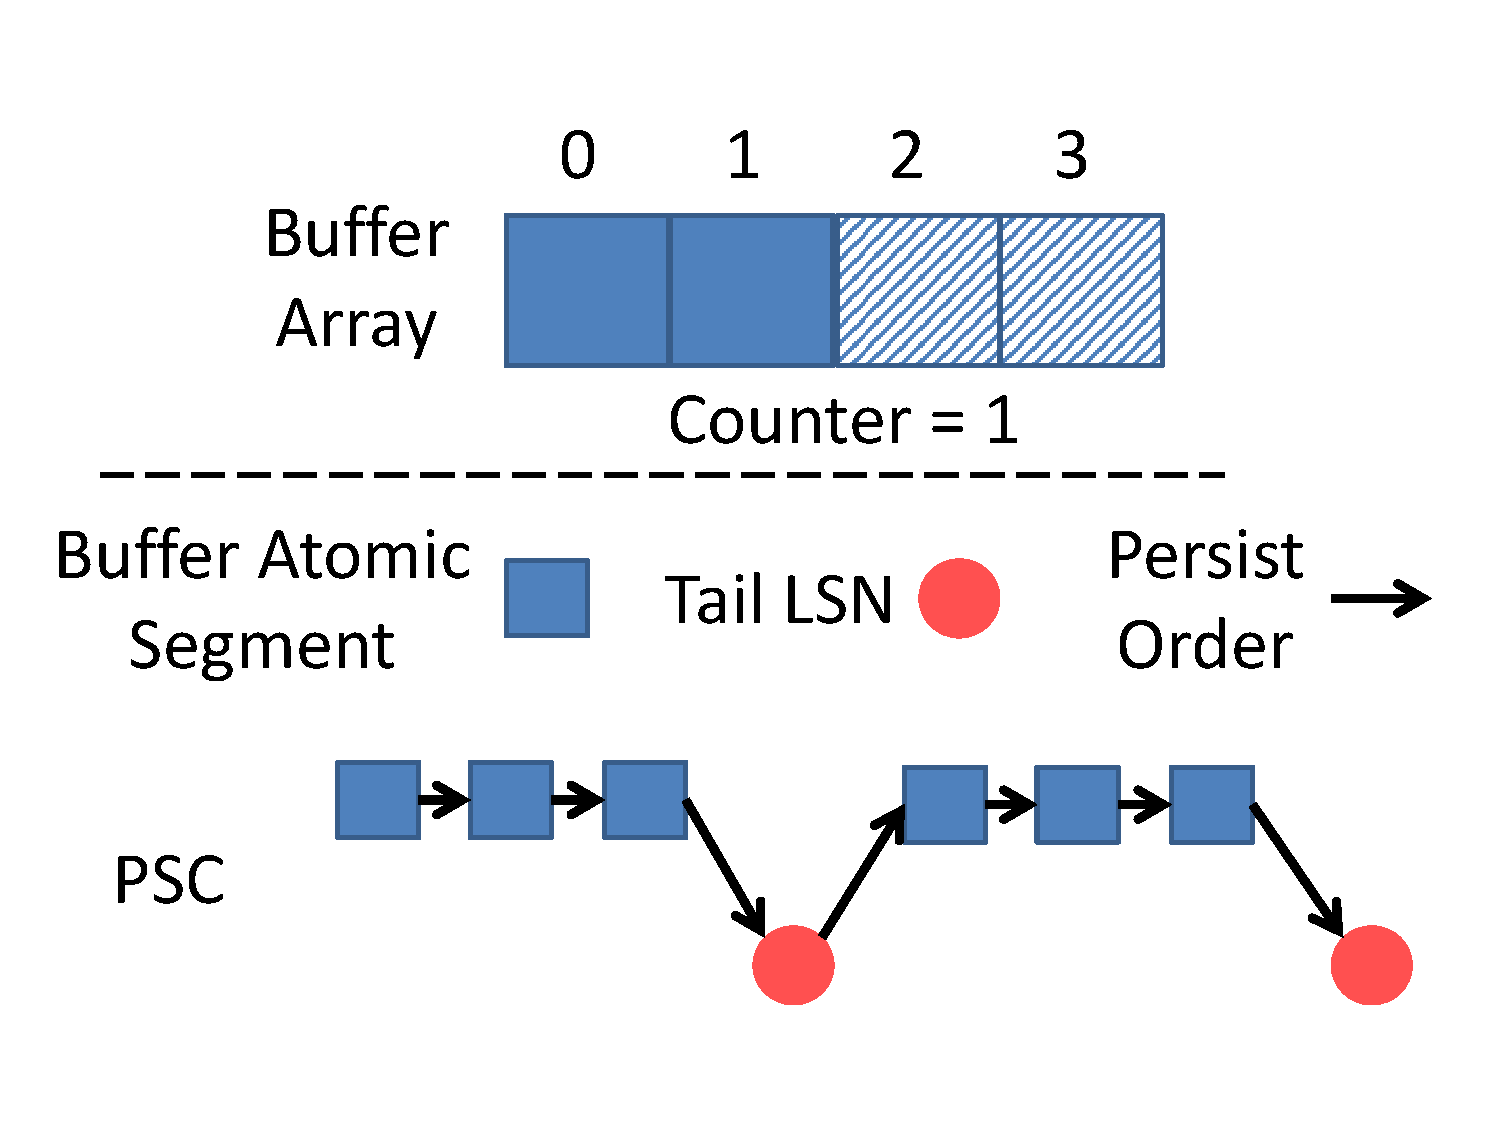
\includegraphics[width=\textwidth]{PMC_patterns/buffer.pdf}
\caption{Persistent buffer. The persistent buffer constists of a persistent array and counter (top).  The array holds persistent data.  The persistent counter marks the greatest persistent slot.  Persisting to the buffer under PSC places depdencies between writing buffer data and updating the counter, as well between persisting the counter and the next buffer persist, forming a chain (bottom).  This occurs both for single threaded and multithreaded use.}
\label{fig:buffer}
\end{figure}


I first discuss a persistent buffer, used as an OLTP database centralized log in \cite{FangHsiao11}.
The version presented here is a simplification of the implementation originally proposed, but illustrates the necessary performance concerns.
This log buffer contains a persistent data array as well as a persistent counter, marking the end of the valid, persistent region of the buffer, shown at the top of Figure~\ref{fig:buffer}.
In the example buffer slots 0 and 1 are persistent and valid, while slots 2 and 3 are not (0 and 1 will be recovered on failure).
For simplicity, I neglect details that require data to wrap around the end of the buffer and instead pretend that the valid region of the buffer always grows from the base offset of the buffer through the address marked by the counter.
Data are inserted into this buffer by acquiring a volatile lock on the structure, reading the counter to determine the next available address, persisting data to that address, and incrementing the counter by the size of the inserted data before releasing the lock.
For correctness, buffer data must persist before the new counter value persists, and all counter values must persist in order.
These dependencies guarantee that, on recovery, the valid portion of the buffer includes the base address through the address located in the persistent counter.

\cite{FangHsiao11} assumes the BPFS consistency model, noting that updates to the counter field will cause each thread to stall while the previous value persists.
Their work provides several complicated optimizations to 1) allow log entries from different threads to persist in parallel (by explicitly removing or re-ordering cross-thread dependencies) and (2) only persist intermediate values of the counter, removing a chain of persist dependencies that would otherwise limit throughput.
Such design improves performance but requires additional effort and is unintuitive.
Other persistent consistency models might enable these optimizations without the use of error-prone software implementations.
I qualitatively evaluation my three consistency models with this buffer, reasoning about persist critical path length per buffer insert.

\textbf{PSC.} Under PSC (recall, persistent sequential consistency) all persists to the buffer and counter form a dependence chain, shown at the bottom of Figure~\ref{fig:buffer}.
Every atomically persistable segment (8 bytes) of buffer data persists in series, followed by the new value of the counter.
The next thread to insert into the buffer reads the counter, a shared variable, ordering all subsequent persists after persists of the previous insert.
Assuming log entries are 100 bytes on average, each insert requires 14 serial persists (13 to persist the log entry data, 1 to persist the counter).
If NVRAM persists take even 100ns (a conservative estimate), entries can only be inserted every 1.4\textmu s, on average (any faster and buffers will eventually fill).
This rate is significantly slower than the throughput of modern concurrent buffers, where cache invalidations take anywhere from tens to hundreds of nanoseconds (multi-core to multi-socket, respectively).
Without relaxed persistent memory consistency models, NVRAM persists will necessarily create a throughput bottleneck.


\begin{figure}
\centering
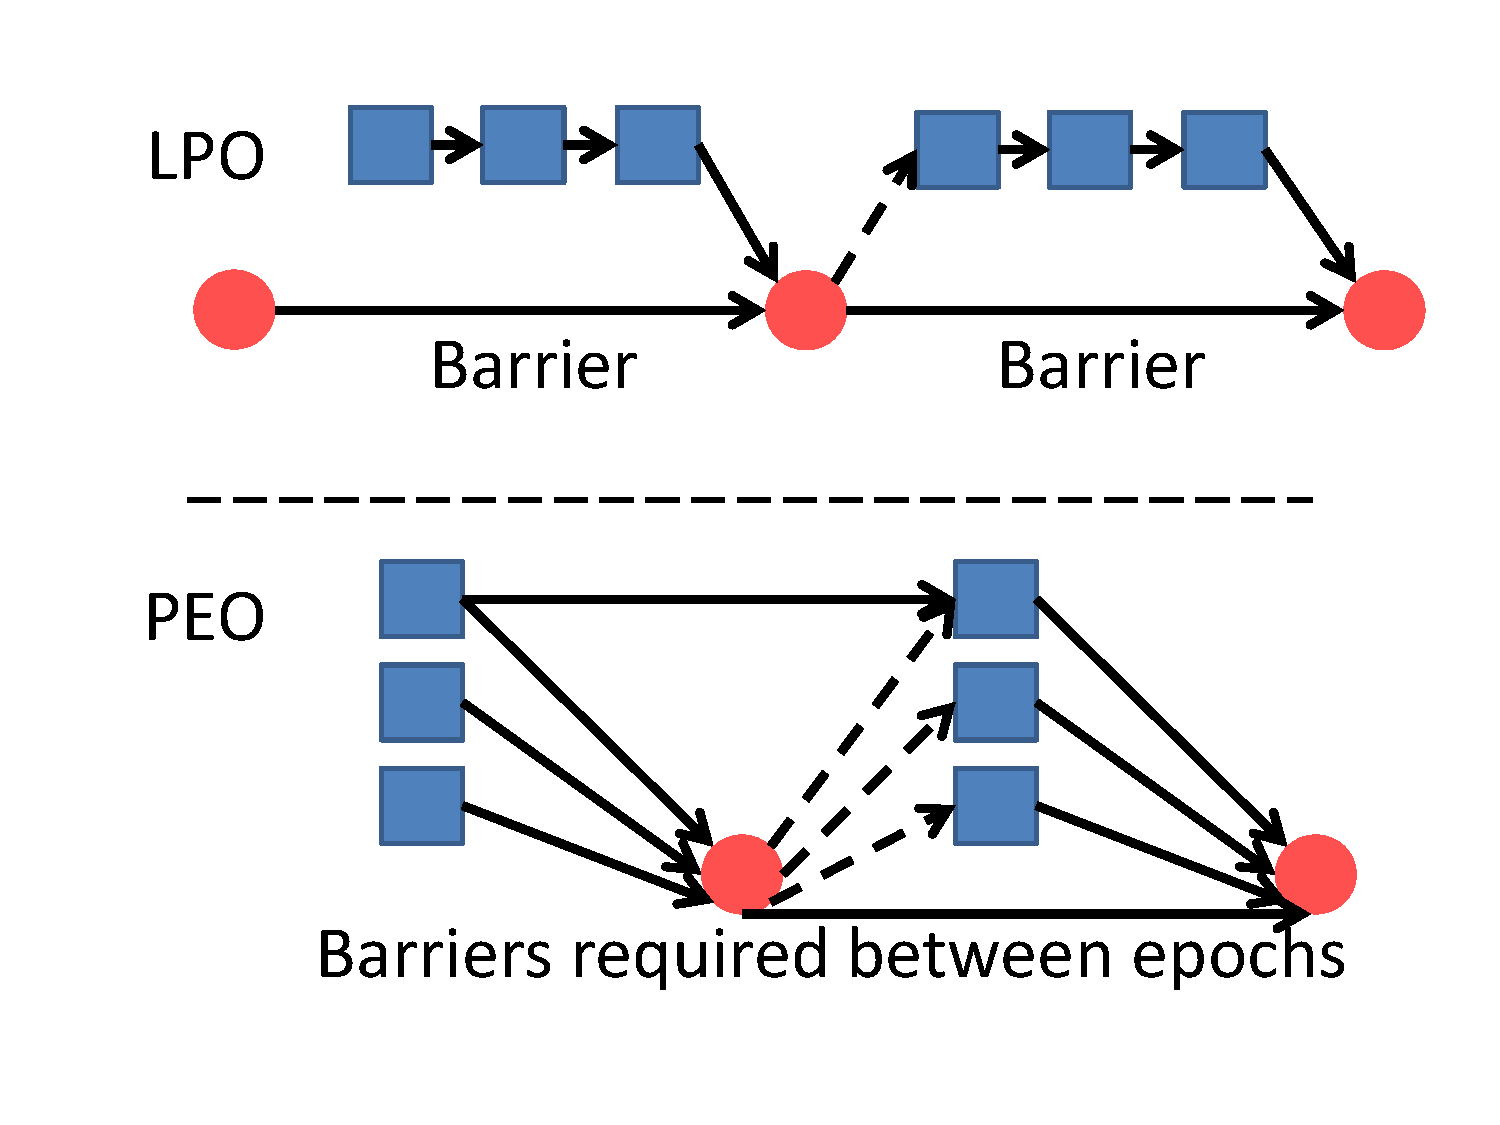
\includegraphics[width=.7\textwidth]{PMC_patterns/buffer_PEO_LPO.pdf}
\caption{\textbf{Buffer execution under LPO and PEO.}  LPO (top) removes persist dependencies between the counter value and subsequent buffer persists on other threads.  Dependencies remain when adjacent buffer inserts are from the same thread (dashed line).  PEO (bottom) allows buffer data to persist in parallel.}
\label{fig:buffer_PEO_LPO}
\end{figure}

\textbf{LPO.} Next I consider the relaxed persistent consistency models introduced in Section~\ref{sec:PMC:PersistenceModels}, starting with LPO.
Recall that LPO (local persist order) enforces program-order persist order within threads, but not cross-thread dependence order (barriers necessary).
Figure~\ref{fig:buffer_PEO_LPO} shows execution of LPO at the top.
Buffer persists continue to serialize and must persist before the counter, but there is no longer a dependence between the counter persisting and later buffer persists from other threads.
Counter values must still persist in-order, which will be enforced with a persist barrier or as a result of persists to the same memory address.
Dependencies \emph{do} exist between counter persists and subsequent buffer persists on the same thread, shown as a dashed line in the Figure.
If every log entry is inserted by a separate thread, LPO results in a persist critical path that involves only counter persists.
However, log entries within a single thread must persist in-order, limiting the throughput of each individual thread.
LPO is easy to program, as all persists within a thread occur-in order, and provides high throughput given sufficient buffering and a large number of threads to yield persist parallelism.

{
\singlespacing
\newsavebox{\BufferPEO}
\begin{lrbox}{\BufferPEO}
  \begin{lstlisting}
PEO:

persist_bar (i)
lock_acquire()
dest = buffer[counter] # reads counter
memcpy(buffer, entry) # persists buffer

persist_bar (ii)
counter += entry.size # persists counter
lock_release()
  \end{lstlisting}
\end{lrbox}

\newsavebox{\BufferTEO}
\begin{lrbox}{\BufferTEO}
  \begin{lstlisting}

TEO:

persist_bar (i)
lock_acquire()

persist_bar (ii)
dest = buffer[counter] # reads counter
memcpy(buffer, entry) # persists buffer

persist_bar (iii)
counter += entry.size # persists counter

persist_bar (iv)
lock_release()
  \end{lstlisting}
\end{lrbox}

\begin{figure}[]
\centering
\subfigure{ \usebox{\BufferPEO} }
\vspace{1 in}
\subfigure{ \usebox{\BufferTEO} }
\caption{\textbf{Buffer insert with PEO/TEO.} Pseudocode implements buffer insert with two persist barriers.  PEO's concurrent epochs allow epoch (ii) to persist in parallel with epoch (i) of the next insert operation. TEO simplifies persist-order reasoning, separating volatile races from persists.  PEO requires four barriers and introduces persist dependencies between persisting buffer data and the previous counter value.}
\label{fig:buffer_PEO_pseudocode}
\end{figure}
}

\textbf{PEO.} The bottom of Figure~\ref{fig:buffer_PEO_LPO} displays buffer execution for PEO -- partial epoch order.
Partial epoch order allows single-thread persists to occur in parallel by placing them in epochs.
Epochs across threads are ordered (or considered concurrent) according to the consistency model and memory sharing.
PEO allows buffer data to persist in parallel, and removes ordering constraints between buffer persists and the previous counter persist from another thread (epochs are concurrent -- see Figure~\ref{fig:buffer_PEO_pseudocode}).
However, buffer persists are ordered after buffer persists of the previous insert (top solid arrow in the Figure), and ordered after counter persists from the same thread (dashed arrows in the Figure).
Even a glance at the Figure reveals how complicated cross-thread dependencies and concurrent persist epochs become.
While PEO provides a correct model by removing deadlocks from BPFS, and enables optimizations by allowing concurrent persist epochs, this is not a reasonable programming interface.

Assuming subsequent inserts occur from different threads, the persist critical path forms a chain of only one persist epoch per insert (either through the counters or through the buffer persists).
Using our earlier assumptions, this model allows inserts every 100ns on average.
Such delays are similar to invalidation delays in modern multi-socket CPU systems, but NVRAM may require more than 100ns per serialized persist.
Furthermore, PEO requires frequent persist barriers, placing a burden on the programmer.
While these epoch barriers are deemed intuitive, they are not as easy to use as sequential consistency (no barriers required).

Reasoning about concurrent epochs is quite difficult.
I provide a second implementation of buffer insert under PEO (Figure~\ref{fig:buffer_PEO_pseudocode}, bottom) that allows a total order of persist epochs (TEO -- as intended by BPFS).
Epochs in this implementation have either volatile races (lock/release) or persists, not both.
Following this rule allows a consistent total order of persist epochs (those epochs that actually persist).
This implementation, while more obviously correct, increases persist critical path by introducing a dependence between counter persist and the next buffer data persist (the dashed arrow of Figure~\ref{fig:buffer_PEO_LPO} implies a dependence even for inserts from different threads).


\begin{figure}
\centering
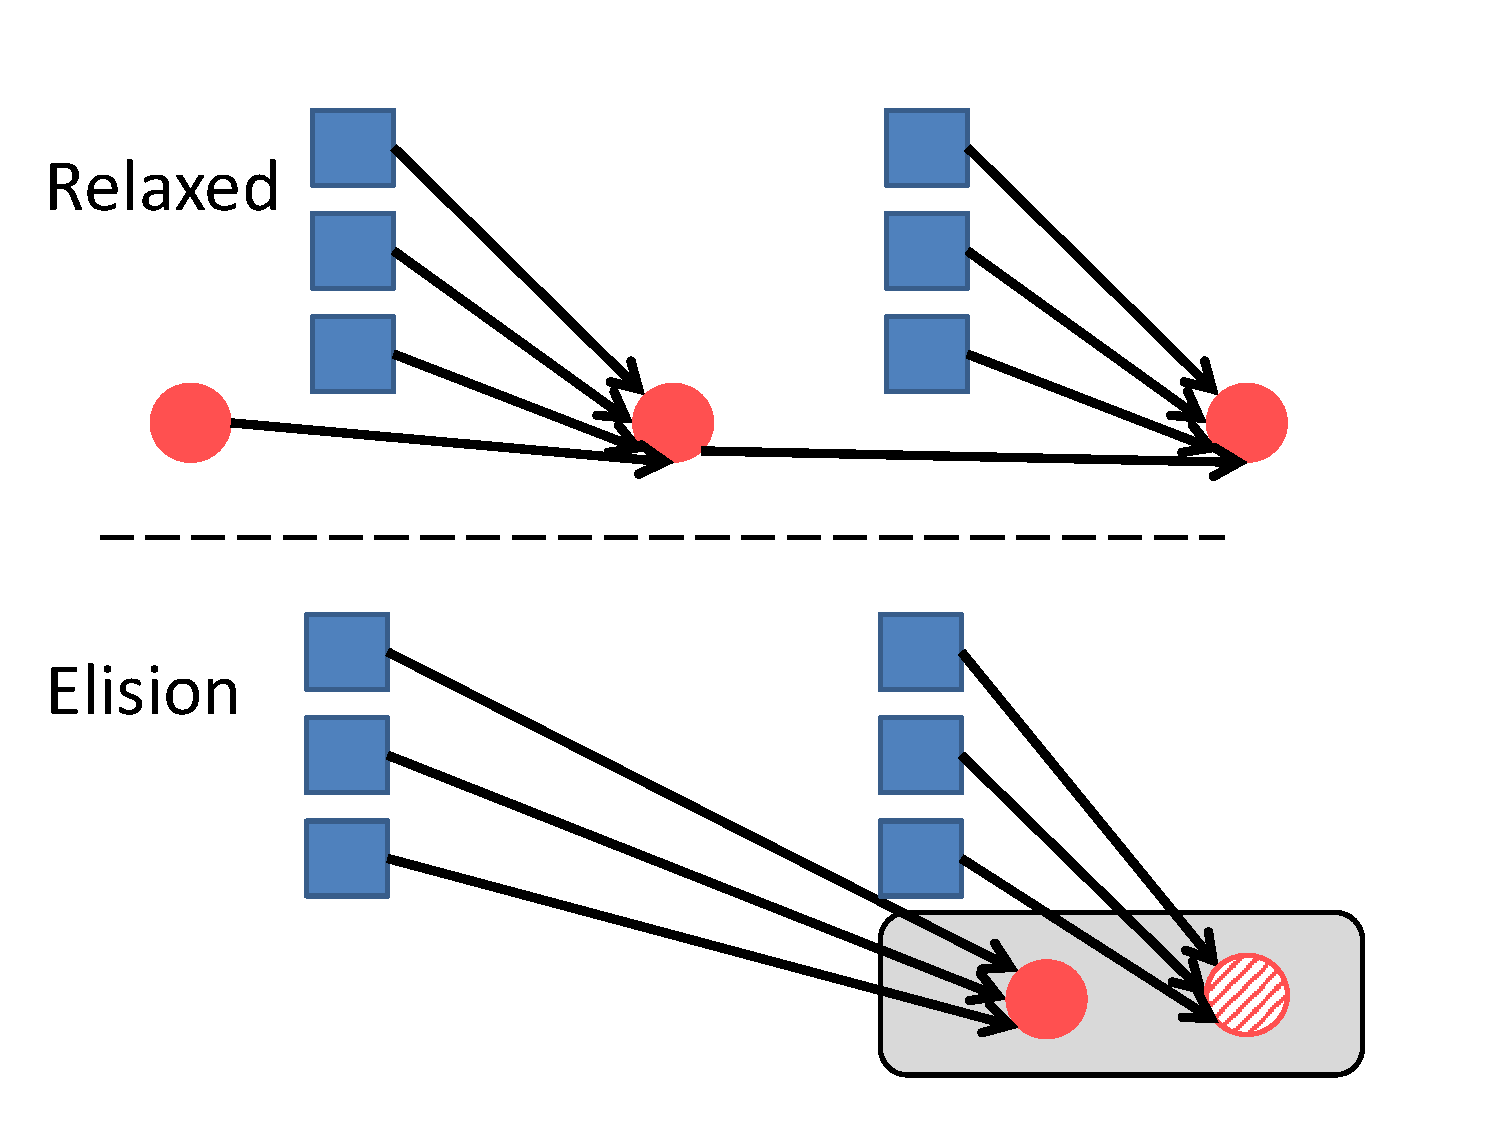
\includegraphics[width=.7\textwidth]{PMC_patterns/buffer_relaxed_elision.pdf}
\caption{\textbf{Buffer execution under relaxed persistent consistency.}  Relaxing persistent consistency removes unnecessary cross-thread dependencies (as in LPO), allows epochs to persist in parallel (as in PEO), and removes unnecessary serial epoch dependencies within threads (top).  Epochs/dependencies are elided by persisting only select counter values (bottom).}
\label{fig:buffer_relaxed_elision}
\end{figure}

\textbf{Relaxed persistent consistency.}
Finally, I imagine a relaxed consistency model for this buffer, shown in Figure~\ref{fig:buffer_relaxed_elision} (top).
I will not describe the semantics of this model, but rather the desired persist dependencies.
Like PEO buffer data persists in parallel.
Like LPO there are no dependencies between counter persists and subsequent buffer persists.
This is true even for single-threaded use.
Doing so requires more complicated barriers that do not impose serial dependencies between epochs, but instead allow precise, possibly named dependencies.
For example, a barrier may declare that an epoch has no earlier persist dependencies, but still enforce that all later epochs persist after it.
Such a barrier would allow a programmer to persist buffer data and guarantee that buffer persists never serialize after counter persists.

I introduce an additional optimization to the relaxed consistency model, leveraging the insight from \cite{FangHsiao11} that not all values must persist, shown at the bottom of Figure~\ref{fig:buffer_relaxed_elision}.
Persistent memory consistency models describe the set of \emph{allowable} persistent states, yet not every allowable state must actually persist.
Since the counter is atomically persistable (8 bytes), the memory system may defer persisting new values.
Once the buffer data for two (or more) adjacent log entries successfully persist, the counter value for the last entry persists (shaded circle in the Figure), implicitly persisting all intermediate counter values at once, eliding persist epochs entirely.
The key is that the counter variable is atomically persistable and is the only persist within its epoch.
We might imagine a new epoch barrier that allows only a single persist of atomic persist size.
This persist defers, hoping to coalesce with similar persist epochs.
A new value eventually persists, but may skip intermediate values so long as all the coalesced persist epochs' dependencies are satisfied.
The result is that the persist critical path is now bounded to a constant -- persists should never limit the throughput of this buffer (assuming large but finite buffers).

More generally, persist dependencies form a schedule or DAG, with persist epochs forming nodes in the graph and epoch dependencies forming edges.
Nodes in the DAG may be combined into an \emph{elision super node} (combining all the nodes' persists) so long as 1) all persists in the super node fit in an atomically persistable size, 2) combining nodes retains the DAG (no cycles introduced), and 3) nodes inherit dependences -- the super node inherits all dependencies of its member nodes, all nodes depending on member nodes now depend on the super node.
An interesting prospect is that as NVRAM technologies progress, the atomically persistable size may increase (say, from 8 bytes to 64 bytes).
Larger atomic persists allow additional persist epochs to coalesce into super nodes, decreasing persist critical path, possibly without user intervention.
It remains unclear if this property should be leveraged by hardware or in the consistency model, if at all.

\section{Persistent Linked List}
\label{sec:PMC_patterns:LinkedList}

\begin{figure}
\centering
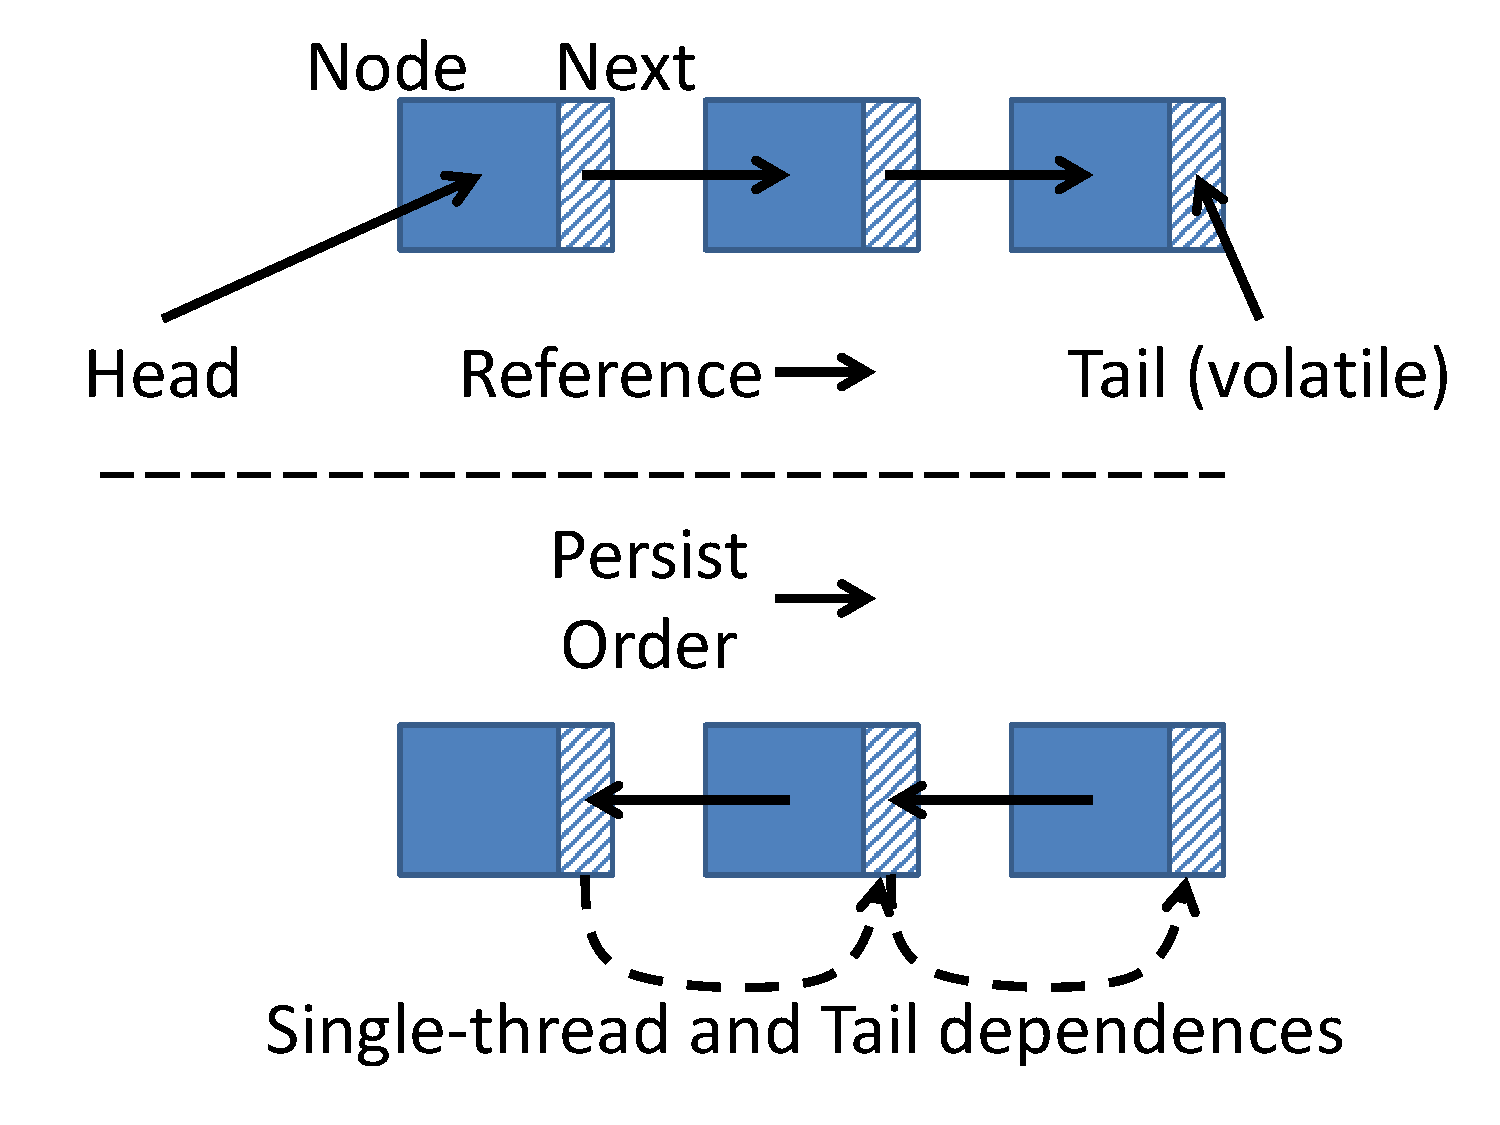
\includegraphics[width=.7\textwidth]{PMC_patterns/linkedlist.pdf}
\caption{\textbf{Persistent linked list.}  The linked list constains nonvolatile Head pointer, volatile Tail pointer, and nodes (data -- solid square; \emph{next} reference -- patterned box).  Nodes persist in parallel (data must still persist before references).  Dashed lines show unnecessary dependencies enforced by strict persistent consistency models, forming a dependence chain.  The valid list is determined at recovery by traversing from Head to the last valid node reference.  Implementing efficient sync remains a challenging.}
\label{fig:LinkedList}
\end{figure}


Finally, I consider a persistent linked list, shown in Figure~\ref{fig:LinkedList}.
The linked list contains a persistent Head reference, persistent nodes (each containing a \emph{next} reference), and a volatile Tail reference to quickly find the end of the list for insertion (although I assume that at recovery the list will only be traversed from the Head).
The top of the figure shows the list, with arrows representing \emph{nexst} references.
Unlike the persistent buffer, where log entries persist in parallel and the counter is overwritten, the linked list does not overwrite any values as new nodes are added.
For correctness, node data must persist before the node \emph{next} reference pointing to that data.

Strict persistent consistency models will enforce that nodes persist in the order they are inserted.
Nodes persist in series, each waiting for the previous node to completely persist (references still persisting after the data they point to).
However, such operation forms a persist dependence chain, limiting persist throughput.
Instead, we would like to allow persist nodes to persist in parallel, yet continue to enforce node data-before-reference persist orders.
The valid portion of the list is determined at recovery by traversing the list from the Head, truncating the list at the first null or invalid reference.

I do not describe how this list likely performs for my persistent consistency models, but simply note the desired behavior.
High performance consistency models will limit persist dependence chains, avoiding the need to persist in series.
However, there is now no efficient way to sync the list.
While we do not constrain the order in which data persists we still need some mechanisms to \emph{observe} when a specific portion of data has persisted -- that is, we must be able to tell when a node and all preceding nodes have persisted.
The programmer may determine that the entire list is persistent (or block until it persists) by traversing the list, adding substantial complexity and overhead.
Thus, this persistent linked list is an interesting design for applications that require high throughput, rarely sync, and require linked lists (to insert or remove nodes from the middle).
Faster, more efficient, yet intuitive sync design remains an interesting challenge.

\section{Conclusion and Future Work}
\label{sec:PMC_patterns:Conclusion}

This chapter considered persistent memory consistency from a performance perspective.
I investigated two simple programming patterns, considering how my proposed persistent consistency models might perform and imagining additional optimizations, separate from the programming model, necessary to increase persistent data structure throughput.

For the future, I would like to develop these ideas and design some sort of methodology to support my claim that persistent memory consistency models are a necessary tool and require further investigation.
To start, I would like to implement the above data structures, annotating the code with persist dependencies and using a timing model similar to the one outlined in Section~\ref{sec:OLTP_design:Methodology}.
Additionally, I would consider implementing these models in Shore-MT.
Finally, I will consider additional models if the described models do not provide sufficient performance, or I discover that other models provide sufficient performance and are easier to program for.
I am especially interested in determining if models stricter than BPFS (fewer barriers) provide sufficient performance.
I plan to submit a paper based on these ideas to this upcoming ISCA, November 2013, and defend next year (2014).

Future work (hopefully outside the scope of my thesis) might consider an evaluation framework that does not require code annotation -- programs are written truly assuming consistency models and executed via simulation.
Additionally, future work will consider actual hardware implementations of useful persistent memory consistency models.
